\section{\secrecdefn}
\label{sec_rec_def_structures}

Many discrete objects, such as sets and graphs, %, and matrices, 
can also be defined recursively. In this section, we look at a variety of examples of recursively-defined structures. While the recursively-defined sequences in \Cref{sec_recursively_defined_sequences} used only one previous term, recursions can involve any number of previous terms.  In this section, we take a sneak peek at such higher order recursions, which we return to explore in more depth in \Cref{sec_fibonacci_higher}.

%%%%%%%%%%%%%%%%%%%%%%%%

\newcommand{\subproperbs}{Proper Bit Strings}
\subsection{\subproperbs}
\label{sub_proper_bit_strings}

We begin with a puzzle. For the sake of this puzzle, we classify each bit string as either proper or improper according to the following definition.

    \begin{defn}[Proper bit strings]
    \label{defn_proper_bs}
    ~
        \begin{apart}
            \item A bit string is \vocab{proper} if it can be constructed from the initial condition \textbf{B} by applying the recursions \textbf{R1} and/or \textbf{R2} a finite number of times each in any order where
                \begin{description}
                    \item [\textbf{~\quad B}:] The empty bit string $\lambda$ is proper.
                    \item [\textbf{~\quad R1}:] If the bit string $b$ is proper, then the bit string $b\bs{0}$ is also proper. 
                    \item [\textbf{~\quad R2}:] If the bit string $b$ is proper, then the bit string $\bs{1}b\bs{1}$ is also proper.
                \end{description} 
                For example, $\bs{1100110}$ is proper, as we show in \Cref{exam_proper_bs} (\ref{part_bs_is_proper}).  
                
            \item All other bit strings are \vocab{improper}. For example, $\bs{011}$ is improper, as we show in \Cref{exam_proper_bs} (\ref{part_bs_is_improper}). 
        \end{apart}
    \end{defn}

Let's verify our examples from \Cref{defn_proper_bs}.

\begin{exam}[Proper bit strings]
\label{exam_proper_bs}
~
    \begin{apart}
        \item \label{part_bs_is_proper} Prove that the bit string $\bs{1100110}$ is proper.
            \begin{soln}
                To see why, we start with the initial condition \textbf{B} that tells us $\lambda$ is proper.  We can use \textbf{R1} to show that $\lambda\bs{0} = \bs{0}$ is proper, and then apply \textbf{R1} again to show that $\bs{00}$ is proper.  Next, we apply \textbf{R2} to show that $\bs{1001}$ is proper, and then apply \textbf{R2} again to show that $\bs{110011}$ is proper.  Finally, we apply \textbf{R1} again to show that $\bs{1100110}$ is proper. 

                We can summarize this series of steps in the diagram: 
                $$ 
                \xrightarrow{\textbf{B}} \lambda \xrightarrow{\textbf{R1}} \bs{0} \xrightarrow{\textbf{R1}} \bs{00} \xrightarrow{\textbf{R2}} \bs{1001} \xrightarrow{\textbf{R2}} \bs{110011} \xrightarrow{\textbf{R1}} \bs{1100110}.$$
            \end{soln}
        \item \label{part_bs_is_improper}  Prove that the bit string $\bs{011}$ is improper.
            \begin{soln}
                We start with \textbf{B} which tells us $\lambda$ is proper.  If we first apply \textbf{R1}, we get that \bs{0} is proper.  To get two more \bs{1}s we can apply \textbf{R2} but that tells us $\bs{101}$ is proper, which is not our bit string.  On the other hand, if we first apply \textbf{R2}, we get that $\bs{11}$ is proper.  To get one \bs{0}, we can apply \textbf{R1} but that tells us \bs{110} is proper, which is also not our bit string.

                Alternatively, we can construct a possibility tree listing all bit strings of length up to three that are proper as shown in \Cref{fig_tree_proper_bs3}.
            \end{soln}
            \begin{figure}[hbtp]
                \centering
                %Used in \Cref{sec_rec_def_structures}

\begin{tikzpicture}[
    grow=right,
    level distance=2.2cm,
    sibling distance=3.8cm,
    every node/.style={anchor=west},
    level 2/.style={sibling distance=2.0cm},
    level 3/.style={sibling distance=1.0cm}
]
\node {$\lambda$}
    child { node {\texttt{11}}
        child { node {\texttt{110}} }
    }
    child { node {\texttt{0}}
        child { node {\texttt{101}} }
        child { node {\texttt{00}}
            child { node {\texttt{000}} }
        }
    };
\end{tikzpicture}
                \caption{All proper bit strings of length three or less}
                \label{fig_tree_proper_bs3}
            \end{figure}
    \end{apart}
\end{exam}

    Now, it is your turn to work with proper bit strings.
    
\begin{act}[Proper Bit Strings Puzzle]
\label{act_proper_bs}
    Recall that a bit string is \vocab{proper} if it can be constructed from these rules in a finite number of steps (and improper otherwise):
                \begin{description}  
                    \item [\textbf{~\quad B}:] The empty bit string $\lambda$ is proper.
                    \item [\textbf{~\quad R1:}] If the bit string $b$ is proper, then the bit string $b\bs{0}$ is also proper. 
                    \item [\textbf{~\quad R2:}] If the bit string $b$ is proper, then the bit string $\bs{1}b\bs{1}$ is also proper.
                \end{description} 
        \begin{actpart}
            \item Explain why the bit string \bs{1010} is proper. That means, show how to use the rules to construct this bit string. 
            \item Explain why the bit string \bs{111010} is proper. Again, show how to use the rules to construct this bit string. 
            \item \label{part_properbs_tree} Draw a possibility tree showing all proper bit strings of length up to four. Underline the bit strings of length four in your tree.
            \item How many proper bit strings of length four are there? 
            \item Use your tree to explain why the bit string \bs{1101} is improper.
            \item How many improper bit strings of length four are there?  Hint: How many bit strings of length four are there (total)? 
            \item Extend to your tree from (\ref{part_properbs_tree}) to show all proper bit strings of length up to five. Draw a box around each bit string of length five in your tree.
            \item How many proper bit strings of length five are there?  How many improper?
        \end{actpart}
\end{act}

Make sure that you have completed \Cref{act_proper_bs} because we are about to reveal some of the answers.

\begin{exam}[Proper bit strings of length up to five.]
\label{exam_proper_bs5}
~
    \begin{apart}
        \item Draw a possibility tree to list all proper bit strings of length up to five.
            \begin{soln}
                We begin with the tree in \Cref{fig_tree_proper_bs3}. Since we only want bit strings of length at most five, we can apply \textbf{R1} and \textbf{R2} to any bit string in that tree, but once we have a bit string of length four we can only apply \textbf{R1}.  The tree is shown in \Cref{fig_tree_proper_bs5}.
            \end{soln}
            \begin{figure}[hbtp]
                \centering
                %Used in \Cref{sec_rec_def_structures}

\begin{tikzpicture}[
    grow=right,
    level distance=2.0cm,
    sibling distance=7.5cm,
    every node/.style={anchor=west},
    level 2/.style={sibling distance=4.0cm},
    level 3/.style={sibling distance=2.3cm},
    level 4/.style={sibling distance=1.3cm},
    level 5/.style={sibling distance=0.9cm}
]
\node {$\lambda$}
    child { node {\texttt{11}}
        child { node {\texttt{1111}}
            child { node {\texttt{11110}} }
        }
        child { node {\texttt{110}}
            child { node {\texttt{11101}} }
            child { node {\texttt{1100}}
                child { node {\texttt{11000}} }
            }
        }
    }
    child { node {\texttt{0}}
        child { node {\texttt{101}}
            child { node {\texttt{11011}} }
            child { node {\texttt{1010}}
                child { node {\texttt{10100}} }
            }
        }
        child { node {\texttt{00}}
            child { node {\texttt{1001}}
                child { node {\texttt{10010}} }
            }
            child { node {\texttt{000}}
                child { node {\texttt{10001}} }
                child { node {\texttt{0000}}
                    child { node {\texttt{00000}} }
                }
            }
        }
    };
\end{tikzpicture}
                \caption{All proper bit strings of length five or less}
                \label{fig_tree_proper_bs5}
            \end{figure}
        \item How many proper bit strings of length five are there?  How many improper bit strings of length five are there? Explain.
            \begin{soln}
                We see in \Cref{fig_tree_proper_bs5} that there are eight proper bit strings of length five. They are
                    $$\bs{00000}, \bs{10001}, \bs{10010}, \bs{10100}, \bs{11011}, \bs{11000}, \bs{11101}, \bs{11110}.$$
                Recall from \Cref{thm_number_bit_strings} that there are $2^5=32$ bit strings of length five.  Therefore, there are $32-8 = 24$ improper bit strings of length five.
            \end{soln}
        \item Explain how we can obtain a list of proper bit strings of length five from the list of proper bit strings of length three and four.
            \begin{soln}
                There are two ways to obtain a proper bit string of length five. 
                
                Case 1: Start with a proper bit string of length four and apply \textbf{R1}.  The proper bit strings of length four are
                    $$\bs{0000}, \bs{1001}, \bs{1010}, \bs{1100}, \bs{1111}$$
                so we get
                    $$\bs{0000\underline{0}}, \bs{1001\underline{0}}, \bs{1010\underline{0}}, \bs{1100\underline{0}}, \bs{1111\underline{0}}.$$
                
                Case 2:  Start with a proper bit string of length three and apply \textbf{R2}. The proper bit strings of length three are
                    $$\bs{000}, \bs{101}, \bs{110}$$
                so we get
                    $$\bs{\underline{1}000\underline{1}}, \bs{\underline{1}101\underline{1}}, \bs{\underline{1}110\underline{1}}$$.
            \end{soln}
    \end{apart}
\end{exam}

Before we look at other recursively-defined structures, we mention how this example connects to computer science.

\begin{defn}[Language]
\label{defn_language}
~
    \begin{apart}
        \item An \vocab{alphabet} is a set of characters. For example, the usual English alphabet $\{a,b,c, \ldots, z\}$ is an alphabet. The set of bits, $\{\bs{0}, \bs{1}\}$, is also an alphabet. 
        \item A \vocab{(formal) language over the alphabet $\Sigma$} is a set of strings where each character of each string is an element of $\Sigma$.  For example, $\mathbb{B}$, the set of all bit strings, is a language over $\Sigma = \{\bs{0}, \bs{1}\}$.  Similarly, $$\mathbb{P} = \{ b \in \mathbb{B} \mid b \text{ is proper}\},$$ is another language over $\Sigma = \{\bs{0}, \bs{1}\}$.
    \end{apart}
\end{defn}

%%%%%%%%%%%%%%%%%%%%%%%%%

\newcommand{\subrecsets}{Recursively-defined Sets}
\subsection{\subrecsets}
\label{sub_rec_def_sets}

In \Cref{act_proper_bs}, we define what it means for a bit string to be proper using a recursion. This example gives rise to the recursively-defined set of proper bit strings.

\begin{exam}[Recursively-defined set of proper bit strings]
\label{exam_rec_def_set_proper_bs}
    Give a recursive definition of the set
        $\mathbb{P} = \{ b \in \mathbb{B} \mid b \text{ is proper}\},$
    where proper bit strings are defined in \Cref{defn_proper_bs}.
            \begin{soln}
                We can rewrite the initial condition and recursions using set notation to obtain:
                    \begin{description} 
                        \item [~\quad \textbf{B}:] $\lambda \in \mathbb{P}$.
                        \item [\textbf{~\quad R1}:] If $b \in \mathbb{P}$, then $b\bs{0}\in \mathbb{P}$. 
                        \item [\textbf{~\quad R2}:] If $b \in \mathbb{P}$, then $\bs{1}b\bs{1}\in \mathbb{P}$.
                    \end{description} 
            \end{soln}
\end{exam}

Let's practice working with proof by mathematical induction to check the unsurprising fact that any bit string consisting of all \bs{0}s is in $\mathbb{P}$.

\begin{exam} [Proof by mathematical induction that involves recursively-defined set]
\label{exam_math_ind_all0s_proper}
    Use mathematical induction (\Cref{pff_math_ind}) to prove that any bit string consisting of all \bs{0}s is in $\mathbb{P}$, the set of all proper bit strings.
        \begin{soln}
            \emph{Proof.}  We induct on $n$, the length of the bit string. 
            
            First, by \textbf{B} we know that $\lambda \in \mathbb{P}$. Next, by \textbf{R1}, it follows that $\lambda \bs{0} = \bs{0} \in \mathbb{P}$.  Thus the bit string of length one consisting of all \bs{0}s is in $\mathbb{P}$.

            Next, assume $b = \underbrace{\bs{000}\cdots\bs{0}}_{n-1 \text{ times}} \in \mathbb{P}$ for some integer $n > 1$.  Then by \textbf{R1}, it follows that $$b\bs{0} = \underbrace{\bs{000}\cdots\bs{0}}_{n-1 \text{ times}}\bs{0} = \underbrace{\bs{000}\cdots\bs{0}}_{n \text{ times}} \in \mathbb{P}.$$
        \end{soln}
\end{exam}

Here is another example of a recursively-defined set.

\begin{exam}[Multiplicative set]
\label{exam_mult_2and3_set}
    Consider the set of integers $L$ constructed recursively as follows:
        \begin{description}
            \item [\textbf{~\quad B1}:] $1 \in L$
            \item [\textbf{~\quad B2}:] $2 \in L$
            \item [\textbf{~\quad B3}:] $3 \in L$
            \item [\textbf{~\quad R}:] If $k,m \in L$, then their product $km \in L$
        \end{description}
    The $L$ consists of all integers that can be formed using \textbf{B1}, \textbf{B2}, \textbf{B3}, and \textbf{R} a finite number of times.  
        \begin{apart}
            \item Is $18 \in L$?  Is $20 \in L$?  Is $1 \in L$? Justify your answers.
                \begin{soln}
                    First, by \textbf{B2} $2 \in L$ and by \textbf{B3} $3 \in L$.  Then, by \textbf{R}, it follows that $(2)(3) = 6 \in L$ and then it follows from \textbf{R} again that $(3)(6)=18 \in L$, so yes.  

                    Next, there is no combination of 2s and 3s that multiply to give 20 because the prime factorization of $20=2^25$.  Therefore there is no way to construct 20, so no. 

                    Last, $1 \in L$ by \textbf{B1}.
                \end{soln}
            \item Give an explicit definition of $L$.
                \begin{soln}
                    Notice that $L$ includes 1 and any integer we can build as a product of 2s and 3s. That is,
                        $$L= \{2^a\cdot 3^b \mid a,b \in \mathbb{N}\}.$$
                \end{soln}
            \item Give an implicit definition of $L$.
                \begin{soln}
                One implicit definition is 
                    $$L = \{ n \in \mathbb{N} \mid n = 2^a\cdot 3^b \text{ for some } a,b \in \mathbb{N}\}$$
                but a more specific implicit definition is
                    $$L = \{ n \in \mathbb{N} \mid \text{if } p \text{ is prime and } p \mid n \text{, then } p=2 \text{ or } p=3\}.$$
                \end{soln}
        \end{apart}
\end{exam}

Your turn to work with a recursively-defined set.

\begin{act}[Additive set]
\label{act_coins_2and3}
    Consider the set $M$ constructed recursively as follows: 
        \begin{description}
            \item [\textbf{~\quad B1:}] $2 \in M$
            \item [\textbf{~\quad B2:}] $3 \in M$
            \item [\textbf{~\quad R:}] If $k,m \in M$, then $k+m \in M$.
        \end{description}   
        \begin{actpart}
            \item \label{part_coins_2and3_build4} Show that $4 \in M$.
            \item Show that $7 \in M$.
            \item Show that $11 \in M$.  
            \item Explain why every positive even integer is in $M$. Hint: How do we get $2k$ for $k \ge 1$?
            \item Explain why any positive odd integer that's greater than or equal to three is in $M$.  Hint: Start with three.  What do you need to add to get $2k+1$ total for $k \ge 1$?
        \end{actpart}
\end{act}

Let's process some of what we learned in \Cref{act_coins_2and3}.

\begin{exam}[Additive set]
\label{exam_coins_2and3}
    Consider the set $M$ constructed recursively in \Cref{act_coins_2and3}.
        \begin{apart}
            \item Explain why $M = \{n \in \mathbb{Z} \mid n \ge 2\}$.
                \begin{soln}
                    We can show any even integer $n \in M$ as follows. Write $n = 2k$ for some integer $k$. By \textbf{B1} we know $2 \in M$. Applying \textbf{R} $(k-1)$ times we get $$ 2 + \underbrace{2+2+\cdots +2}_{k-1 \text{ times}} \in M.$$
                    But $$2 + \underbrace{2+2+\cdots +2}_{k-1 \text{ times}} = 2+ 2(k-1) = 2k =n.$$ Thus $n \in M$.

                    We can show any odd integer $n \in M$ for $n \ge 3$ as follows.  Write $n = 2k+1$ for some integer $k$. Since $n \ge 3$, it follows that $k \ge 1$.  By \textbf{B2} we know $3 \in M$. Applying \textbf{R} $(k-1)$ times we get $$ 3 + \underbrace{2+2+\cdots +2}_{k-1 \text{ times}} \in M.$$
                    But $$3 + \underbrace{2+2+\cdots +2}_{k-1 \text{ times}} = 3 + 2(k-1) = 2k + 1=n.$$ Thus $n \in M$.
                \end{soln}
            \item \label{part_math_ind_coins_2and3} Use mathematical induction to verify that $n \in M$ for any integer $n \ge 2$.
                \begin{soln}
                    \emph{Proof.}  Induct on $n$.  

                    First, when $n = 2$, we know $2 \in M$ by \textbf{B}.

                    Next, assume $n-1 \in M$ for some $n >1$.  We consider two cases.

                    Case 1: Somewhere in the process of constructing $n-1$ we used \textbf{B1}.  That is, $n-1=2+m$ for some $m \in M$.  Adding one to each side of the equation we get $n = 3 + m$, and so $n$ can be constructed from $m$ using \textbf{B2} and \textbf{R}.

                    Case 2: Nowhere in the process of constructing $n-1$ did we use \textbf{B1}.  It follows that somewhere in the process of constructing $n-1$ we used \textbf{B2}. That is, $n-1 = 3+m$ for some $m \in M$.  Adding one to each side of the equation we get $n = 4 + m$, and so $n$ can be constructed from $m$ using \textbf{B1} twice and \textbf{R}. 
                \end{soln}
        \end{apart}
\end{exam}

In many textbooks, the example from \Cref{act_coins_2and3} is described in terms of coins or stamps.  In that vocabulary, we can make any value of money 2{\textcent} or greater using 2{\textcent} and 3{\textcent} coins, or any postage 2{\textcent} or greater using 2{\textcent} and 3{\textcent} stamps.

%%%%%%%%%%%%%%%%%%%%%%%%

\newcommand{\subrecgraphs}{Recursively-defined Graphs} % and Matrices}
\subsection{\subrecgraphs}
\label{sub_rec_def_graphs}

We begin with an activity.

\begin{act}[Lopsided trees]
\label{act_rec_trees}
    We define the family of \vocab{lopsided trees}, $T_n$, as follows:  $T_1$ and $T_2$ are each just a single root vertex. For $n\ge3$, the lopsided tree $T_n$ is built from the trees $T_{n-1}$ (drawn on the left) and $T_{n-2}$ (drawn on the right) by adding a new root vertex, an edge between the new root vertex and the root vertex of $T_{n-1}$, and an edge between the new root vertex and the root vertex of $T_{n-2}$, as represented schematically in \Cref{figure_rec_trees_defn}.  
        \begin{figure}[hbtp]
            \centering
            %Used in \Cref{oact_rec_trees}.

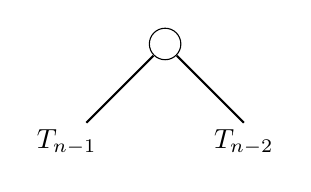
\begin{tikzpicture} 
    [scale =.5]
    \GraphInit[vstyle=Welsh]
    \SetGraphUnit{2}
    \draw (2,2) circle [radius=.4,thick];
    \draw (0,0) to (1.7,1.7)[thick];
    \draw (4,0) to (2.3,1.7)[thick];
    \node at (-0.5,-0.5) {$T_{n-1}$};
    \node at (4,-0.5) {$T_{n-2}$};
\end{tikzpicture}
            \caption{Defining the lopsided tree $T_n$ from \Cref{act_rec_trees}.}
            \label{figure_rec_trees_defn}
        \end{figure}
    
    The first five lopsided trees are drawn in \Cref{figure_rec_trees_first_four}.
        \begin{figure}[hbtp]
            \centering
            %Used in \Cref{oact_rec_trees}.

\begin{tikzpicture} 
    [scale =.5]
    \GraphInit[vstyle=Welsh]
    \SetGraphUnit{2}
    \SetVertexNoLabel
    %T1
    \Vertex[x=0,y=6]{a}
    %T2
    \Vertex[x=4,y=6]{b}
    %T3
    \Vertex[x=10,y=6]{c}
        %Left
        \Vertex[x=9,y=4]{p}
        % Right
        \Vertex[x=11,y=4]{q}
        \Edges(p,c,q)
    %T4
    \Vertex[x=18,y=6]{d}
        %Left
        \Vertex[x=17,y=4]{r}
            %Subleft
            \Vertex[x=16,y=2]{w}
            %Subright
            \Vertex[x=18,y=2]{x} 
            \Edges(w,r,x)
        % Right
        \Vertex[x=19,y=4]{s}
        \Edges(r,d,s)
    %T5
    \Vertex[x=28,y=6]{e}
        %Left
        \Vertex[x=26,y=4]{t}
            %Subleft
            \Vertex[x=25,y=2]{y}
                %Subsubleft
                    \Vertex[x=24,y=0]{i}
                %Subsubright
                    \Vertex[x=26,y=0]{j}   
                    \Edges(i,y,j)
            %Subright
            \Vertex[x=27,y=2]{z} 
            \Edges(y,t,z)
        % Right
        \Vertex[x=30,y=4]{u}
            %Left
            \Vertex[x=29,y=2]{m}
            %Left
            \Vertex[x=31,y=2]{n}
            \Edges(m,u,n)
        \Edges(t,e,u)   
\end{tikzpicture}
%
% ~ \hspace{.25in} ~%%%%
% %
% \begin{tikzpicture} %T2
%     [scale =.5]
%     \GraphInit[vstyle=Welsh]
%     \SetGraphUnit{2}
%     \SetVertexNoLabel
    
% \end{tikzpicture}
% %
% ~ \hspace{.25in} ~%%%%
% %
% \begin{tikzpicture} %T3
%     [scale =.5]
%     \GraphInit[vstyle=Welsh]
%     \SetGraphUnit{2}
%     \SetVertexNoLabel
%     \Vertex[x=0,y=2]{r}
%     \Vertex[x=-1,y=0]{c}
%     \Vertex[x=1,y=0]{d}
%     \Edges(c,r,d)
% \end{tikzpicture}
% %
% ~ \hspace{.25in} ~%%%%
% %
% \begin{tikzpicture}%T4
%     [scale =.5]
%     \GraphInit[vstyle=Welsh]
%     \SetGraphUnit{2}
%     \SetVertexNoLabel
%     %root
%     \Vertex[x=0,y=4]{r}
%     %left
%     \Vertex[x=-1,y=2]{c}
%     \Vertex[x=-2,y=0]{w}
%     \Vertex[x=0,y=0]{x}
%     %right
%     \Vertex[x=1,y=2]{d}
%     \Edges(c,r,d)
%     \Edges(w,c,x)
% \end{tikzpicture}
% %
% ~ \hspace{.25in} ~%%%%
% %
% \begin{tikzpicture}%T5
%     [scale =.5]
%     \GraphInit[vstyle=Welsh]
%     \SetGraphUnit{2}
%     \SetVertexNoLabel
%     % root
%     \Vertex[x=2,y=6]{a}
%     % left
%     \Vertex[x=0,y=4]{r}
%     %sub left    
%     \Vertex[x=0,y=0]{x}
%     \Vertex[x=-1,y=2]{c}
%     \Vertex[x=1,y=2]{d}
%     %sub right
%     \Vertex[x=-2,y=0]{w}
%     % right
%     \Vertex[x=4,y=4]{s}
%     %sub left
%     \Vertex[x=3,y=2]{e}
%     % sub right
%     \Vertex[x=5,y=2]{f}
%     \Edges(r,a,s)
%     \Edges(c,r,d)
%     \Edges(w,c,x)
%     \Edges(e,s,f)
% \end{tikzpicture}
            \caption{From left to right: the lopsided trees $T_1$, $T_2$, $T_3$, $T_4$, an $T_5$ from \Cref{act_rec_trees}.}
            \label{figure_rec_trees_first_four}
        \end{figure}
        \begin{actpart}
            \item Copy $T_5$ and explain how $T_3$ and $T_4$ were used to create $T_5$.
            \item Draw $T_6$.  Pay attention to what is on the left versus the right in your drawing. 
            \item Recall that leaf is a vertex of degree one.  Write $w_n=$ the number of leaves in the lopsided tree $T_n$ for $n \ge 3$.  Explain why $w_3=2$ and $w_4=3$.
            \item Calculate $w_5$ and $w_6$.
            \item \label{part_rec_trees_leaves} Write an recursive definition of the sequence $w_n$  and explain why the equation holds by referring to the trees (not just the numbers you found).  Hint: The definition uses the two previous terms.
        \end{actpart}
\end{act}

Let's take a closer look at the trees from \Cref{act_rec_trees}.

\begin{exam}[Lopsided trees]
\label{exam_lopsided_trees}
    In \Cref{act_rec_trees}, we defined the family of lopsided trees $T_n$.  Write $w_n=$ the number of leaves in the lopsided tree $T_n$ for $n \ge 3$.
        \begin{apart}
            \item Make a table showing the values of $w_n$ for $n=1,2,3,4,5,6$.
                \begin{soln}
                    We can count the leaves in the graphs in \Cref{figure_rec_trees_first_four} for $n=1,2,3,4,5$.  For $n=6$ note that the leaves in $T_6$ consists of the leaves from $T_5$ (on the left) and the leaves from $T_6$ (on the right).  Thus $w_6 = w_5 + w_4 = 5+3=8$.  We summarize our findings in \Cref{tab_leaves_lopsided}.
                \end{soln}
                \begin{table}[hbtp]
                    \centering
                    \begin{tabular}{c|c|c|c|c|c|c|c}
                        $n$ & 1 & 2 & 3 & 4 & 5 & 6 \\
                        $w_n$ & 1 & 1 & 2 & 3 & 5 & 8 
                    \end{tabular}
                    \caption{The number of leaves in the lopsided trees.}
                    \label{tab_leaves_lopsided}
                \end{table}
            \item Write a recursive definition for $w_n$ for $n \ge 1$, including the initial conditions.
                \begin{soln}
                    Since the leaves in $T_n$ are the leaves from $T_{n-1}$ (on the left) and the leaves from $T_{n-2}$ (on the right), we get 
                        $$w_n=w_{n-1}+w_{n-2}$$
                    for $n \ge 3$.  The initial conditions are $w_1=1$ and $w_2=1$.  Since the recursion uses two previous terms, we need two initial conditions to start.
                \end{soln}
        \end{apart}
\end{exam}

The lopsided trees in \Cref{act_rec_trees} were defined recursively.  Here is another example of a recursively-defined family of graphs.

\begin{exam}[Recursive definition of the path graphs]
\label{exam_rec_path_graphs}
    Consider the path graphs $P_n$.  We can define these graphs recursively setting $P_1$ to be a single vertex and then $P_n$ is formed from $P_{n-1}$ by adding one new vertex and an edge connecting that new vertex to one of the end vertices of $P_{n-1}$.  
    \begin{actpart}
        \item Use this definition to draw the first five path graphs.
            \begin{soln}
            The first five path graphs are drawn in \Cref{figure_path_graphs_recursive}.
                \begin{figure}[hbtp]
                    \centering
                    %Used in \Cref{sub_seq_recursive} \Cref{exam_rec_path_graphs}

$P_1$
\begin{tikzpicture}
[scale =.5]
\GraphInit[vstyle=Welsh]
\SetGraphUnit{2}
\SetVertexNoLabel
\Vertex[LabelOut,Lpos=90,x=0,y=0]{$A$}
\end{tikzpicture}
\hspace{.15in}
$P_2$
\begin{tikzpicture}
[scale =.5]
\GraphInit[vstyle=Welsh]
\SetGraphUnit{2}
\SetVertexNoLabel
\Vertex[LabelOut,Lpos=90,x=0,y=0]{$A$}
\Vertex[LabelOut,Lpos= 90,x=2,y=0]{$B$}
\Edges($A$, $B$)
\end{tikzpicture}
\hspace{.15in}
$P_3$
\begin{tikzpicture}
[scale =.5]
\GraphInit[vstyle=Welsh]
\SetGraphUnit{2}
\SetVertexNoLabel
\Vertex[LabelOut,Lpos=90,x=0,y=0]{$A$}
\Vertex[LabelOut,Lpos= 90,x=2,y=0]{$B$}
\Vertex[LabelOut,Lpos= 90,x=4,y=0]{$C$}
\Edges($A$, $B$, $C$)
\end{tikzpicture}
\vspace{.25in}

$P_4$
\begin{tikzpicture}
[scale =.5]
\GraphInit[vstyle=Welsh]
\SetGraphUnit{2}
\SetVertexNoLabel
\Vertex[LabelOut,Lpos=90,x=0,y=0]{$A$}
\Vertex[LabelOut,Lpos= 90,x=2,y=0]{$B$}
\Vertex[LabelOut,Lpos= 90,x=4,y=0]{$C$}
\Vertex[LabelOut,Lpos= 90,x=6,y=0]{$D$}
\Edges($A$, $B$, $C$,$D$)
\end{tikzpicture}
\hspace{.15in}
$P_5$
\begin{tikzpicture}
[scale =.5]
\GraphInit[vstyle=Welsh]
\SetGraphUnit{2}
\SetVertexNoLabel
\Vertex[LabelOut,Lpos=90,x=0,y=0]{$A$}
\Vertex[LabelOut,Lpos= 90,x=2,y=0]{$B$}
\Vertex[LabelOut,Lpos= 90,x=4,y=0]{$C$}
\Vertex[LabelOut,Lpos= 90,x=6,y=0]{$D$}
\Vertex[LabelOut,Lpos= 90,x=8,y=0]{$E$}
\Edges($A$, $B$, $C$,$D$,$E$)
\end{tikzpicture}
                    \caption{The path graphs}
                    \label{figure_path_graphs_recursive}
                \end{figure}
            \end{soln}
        \item Write a recursive definition for $v_n=$ the number of vertices of $P_n$ and $e_n=$ the number of edges of $P_n$.
            \begin{soln}
                First, $P_1$ has one vertex and zero edges so $v_1=1$ and $e_1=0$.  Next, at each step we add one new vertex and so the number of new vertices is 1 more than the number of old vertices.  That is, $v_n=v_{n-1}+1$ for $n \ge 2$.  Similarly, at each step we add one new edge and so the number of new edges is 1 more than the number of old edges. That is, $e_n=e_{n-1}+1$ for $n \ge 2$. Notice that $v$ and $e$ are defined using the same recursive rule but  because they have different initial conditions we get different sequences.  In fact, $v_n=n$ and $e_n=n-1$ for $n \ge 1$.
            \end{soln}
        \item Determine the adjacency matrices for $P_1$, $P_2$, $P_3$, $P_4$, and $P_5$. Then describe how the adjacency matrix for $P_n$ can be constructed from the adjacency matrix for $P_{n-1}$.
            \begin{soln}
                \Cref{fig_paths12345_labeled} shows labeled versions of the path graphs $P_1$, $P_2$, $P_3$, $P_4$, and $P_5$.

                    \begin{figure}
                        \centering
                        %Used in \Cref{sec_recursively_defined_sequences}

% P1
\begin{tikzpicture}
    [scale =.5]
    \GraphInit[vstyle=Welsh]
    \SetGraphUnit{2}
    %\SetVertexNoLabel
    \Vertex[LabelOut,Lpos=-90,x=0,y=0]{$v_1$}
\end{tikzpicture}
%
\hspace{.15in} %%%%
%
% P2
\begin{tikzpicture}
    [scale =.5]
    \GraphInit[vstyle=Welsh]
    \SetGraphUnit{2}
    %\SetVertexNoLabel
    \Vertex[LabelOut,Lpos=-90,x=0,y=0]{$v_1$}
    \Vertex[LabelOut,Lpos=-90,x=2,y=0]{$v_2$} 
    \Edges($v_1$, $v_2$)
\end{tikzpicture}
%
\hspace{.15in} %%%%
%
% P3
\begin{tikzpicture}
    [scale =.5]
    \GraphInit[vstyle=Welsh]
    \SetGraphUnit{2}
    %\SetVertexNoLabel
    \Vertex[LabelOut,Lpos=-90,x=0,y=0]{$v_1$}
    \Vertex[LabelOut,Lpos=-90,x=2,y=0]{$v_2$} 
    \Vertex[LabelOut,Lpos=-90,x=4,y=0]{$v_3$}
    \Edges($v_1$, $v_2$, $v_3$)
\end{tikzpicture}
%
\hspace{.15in} %%%%
%
% P4
\begin{tikzpicture}
    [scale =.5]
    \GraphInit[vstyle=Welsh]
    \SetGraphUnit{2}
    %\SetVertexNoLabel
    \Vertex[LabelOut,Lpos=-90,x=0,y=0]{$v_1$}
    \Vertex[LabelOut,Lpos=-90,x=2,y=0]{$v_2$} 
    \Vertex[LabelOut,Lpos=-90,x=4,y=0]{$v_3$}
    \Vertex[LabelOut,Lpos=-90,x=6,y=0]{$v_4$}
    \Edges($v_1$, $v_2$, $v_3$, $v_4$)
\end{tikzpicture}
%
\hspace{.15in} %%%%
%
% P5
\begin{tikzpicture}
    [scale =.5]
    \GraphInit[vstyle=Welsh]
    \SetGraphUnit{2}
    %\SetVertexNoLabel
    \Vertex[LabelOut,Lpos=-90,x=0,y=0]{$v_1$}
    \Vertex[LabelOut,Lpos=-90,x=2,y=0]{$v_2$} 
    \Vertex[LabelOut,Lpos=-90,x=4,y=0]{$v_3$}
    \Vertex[LabelOut,Lpos=-90,x=6,y=0]{$v_4$}
    \Vertex[LabelOut,Lpos=-90,x=8,y=0]{$v_5$}
    \Edges($v_1$, $v_2$, $v_3$, $v_4$,$v_5$)
\end{tikzpicture}
                        \caption{Paths $P_1$, $P_2$, $P_3$, $P_4$, and $P_5$ labeled.}
                        \label{fig_paths12345_labeled}
                    \end{figure}

                The corresponding adjacency matrices are shown in \Cref{tab_adj_mat_paths}.  Starting with $P_{n-1}$ we add a new column on the far right and a new row at the bottom which are all \bs{0}s except the next to last entry in the column and row is \bs{1}.

            \end{soln}
            \begin{table}[htbp]
                \centering
                \begin{tabular} {cc}
                    & $\begin{array} {c} v_1\end{array}$ \\ 
                    $\begin{array}{r} v_1\end{array}$  
                    & $\left[ \begin{array} {cccccc} 
                    ~\bs{0}~  \\
                    \end{array} \right]$ \\
                \end{tabular}
                \hspace{.15in}
                \begin{tabular} {cc}
                    & $\begin{array} {cc} v_1&v_2 \end{array}$ \\ 
                    $\begin{array}{r} v_1 \\ v_2 \end{array}$  
                    & $\left[ \begin{array} {cccccc} 
                    ~\bs{0}~ & ~\bs{1}~  \\
                    \bs{1} & \bs{0}  \\
                    \end{array} \right]$ \\
                \end{tabular}
                \hspace{.15in}
                \begin{tabular} {cc}
                    & $\begin{array} {ccc} v_1&v_2&v_3 \end{array}$ \\ 
                    $\begin{array}{r} v_1 \\ v_2 \\ v_3 \end{array}$  
                    & $\left[ \begin{array} {cccccc} 
                    ~\bs{0}~ & ~\bs{1}~ & ~\bs{0}~ \\
                    \bs{1} & \bs{0} & \bs{1} \\
                    \bs{0} & \bs{1} & \bs{0} \\
                    \end{array} \right]$ \\
                \end{tabular}
                \hspace{.15in}
                \begin{tabular} {cc}
                    & $\begin{array} {cccc} v_1&v_2&v_3&v_4 \end{array}$ \\ 
                    $\begin{array}{r} v_1 \\ v_2 \\ v_3 \\v_4 \end{array}$  
                    & $\left[ \begin{array} {cccccc} 
                    ~\bs{0}~ & ~\bs{1}~ & ~\bs{0}~ & ~\bs{0}~\\
                    \bs{1} & \bs{0} & \bs{1} & \bs{0} \\
                    \bs{0} & \bs{1} & \bs{0} & \bs{1} \\
                    \bs{0} & \bs{0} & \bs{1} & \bs{0} \\
                    \end{array} \right]$ \\
                \end{tabular}
                \hspace{.15in}
                \begin{tabular} {cc}
                    & $\begin{array} {ccccc} v_1&v_2&v_3&v_4&v_5 \end{array}$ \\ 
                    $\begin{array}{r} v_1 \\ v_2 \\ v_3 \\v_4\\v_5 \end{array}$  
                    & $\left[ \begin{array} {cccccc} 
                    ~\bs{0}~ & ~\bs{1}~ & ~\bs{0}~ & ~\bs{0}~& ~\bs{0}~\\
                    \bs{1} & \bs{0} & \bs{1} & \bs{0} & \bs{0}\\
                    \bs{0} & \bs{1} & \bs{0} & \bs{1} & \bs{0}\\
                    \bs{0} & \bs{0} & \bs{1} & \bs{0} & \bs{1}\\
                    \bs{0} & \bs{0} & \bs{0} & \bs{1} & \bs{0}\\
                    \end{array} \right]$ \\
                \end{tabular}
                \caption{The adjacency matrices for the paths $P_1$, $P_2$, $P_3$, $P_4$, and $P_5$.}
                \label{tab_adj_mat_paths}
            \end{table}

    \end{actpart}
    \end{exam}

%SU:  Would like to have recursive matrices too.  Revisit adjacency matrices here.

%%%%%%%%%%%%%%%%%%%%%%%%

\subsection{Exercises}

%%%%%%%%%%%%%%%%%%%%%%%%

\subsubsection*{Exercises for \Cref{sub_proper_bit_strings} \subproperbs}

\begin{exer}[\exerP] % improper bit string example]
\label{exer_improperbs_example}
~
    \begin{exerpart}
        \item Explain why the bit string \bs{101111} is improper.  
        \item Explain why the bit string \bs{1011111} is improper.  Consider the case where you start with \textbf{R1} and the case where you start with \textbf{R2}.
    \end{exerpart}
\end{exer}

\begin{exer}[\exerU] % proper bit strings of length 6]
\label{exer_properbs_length6}
    In \Cref{fig_tree_proper_bs5}, we drew a possibility tree showing all proper bit strings of length up to five.  
    \begin{exerpart}
        \item Use the list of proper bit strings of length four and length five from \Cref{exam_proper_bs5} to generate a list of all proper bit strings of length six.  
        \item How many proper bit strings of length six are there?
        \item \label{part_properbs_count6_from4and5} How does the number of proper bit strings of length six relate to the number of proper bit strings of length four and the number of proper bit strings of length five?
    \end{exerpart} 
\end{exer}

\begin{exer}[\exerU] % counting proper and improper bit strings]
\label{exer_properbs_count}
    Generalize your observation from \Cref{exer_properbs_length6}(\ref{part_properbs_count6_from4and5}) to write a recursive definition of the sequence $p_n=$ the number of proper bit strings of length $n$, including initial conditions. 
\end{exer}

\begin{exer}[\exerR] % proper bit strings
\label{exer_dyk_proper_bs}
    Do you know \ldots
        \begin{exerpart}
            \item How to use a recursive definition of a language?
            \item How to draw a possibility tree to list strings from a recursively-defined language?
            \item How to recursively define a sequence using two previous terms and why we need two initial conditions?
        \end{exerpart}
\end{exer}

\begin{exer}[\exerE] % proper bit string conjectures]
\label{exer_properbs_examples}
    In this problem, we are looking for general conjectures that tell us if a bit string is proper or improper by looking at it-- meaning without working through the rules, drawing a tree, considering cases, or anything complicated.  Your conjectures should be in the form
        \begin{quote}
            If a bit string is/has \underline{\hspace{1in}}, then it is automatically proper/improper.
        \end{quote}
    Your conjectures should not be examples, they should be general rules that apply to an infinite number of bit strings. 
    \begin{exerpart}
        \item Make a conjecture about a condition that automatically shows a bit string is proper.
        \item Make another conjecture about a condition that automatically shows a bit string is proper.
        \item Make a conjecture about a condition that automatically shows a bit string is improper.
    \end{exerpart}
\end{exer}

\begin{exer}[\exerE] % proper bit string start]
\label{exer_properbs_start}
~
    \begin{exerpart}
        \item Describe in detail a simple process that determines whether a proper bit string was constructed starting with \textbf{R1} or starting with \textbf{R2}. This process should not involve testing all possible constructions.
        \item Extend your process from \Cref{exer_properbs_start} to describe in detail a relatively simple process that determines whether a bit string is proper or improper.  This process should not involve testing all possible constructions.
    \end{exerpart}   
\end{exer}

%%%%%%%%%%%%%%%%%

\subsubsection*{Exercises for \Cref{sub_rec_def_sets}
\subrecsets}

\begin{exer}[\exerP] % 3s and 5s additive set]
\label{exer_coins_3and5_set}
    Consider the set $M$ constructed recursively as follows:      
        \begin{description}
            \item [\textbf{~\quad B1:}] $3 \in M$
            \item [\textbf{~\quad B2:}] $5 \in M$
            \item [\textbf{~\quad R:}] If $k,m \in M$, then $k+m \in M$.
        \end{description} 
        \begin{exerpart}
             \item Show that $8 \in M$, $9 \in M$, and $10 \in M$.
             \item Which of $1, 2, 3, 4, 5, 6, 7$ are in $M$?  Briefly justify your answers.        
         \end{exerpart}
\end{exer}

\begin{exer}[\exerU] % 3s and 5s additive set building larger values]
\label{exer_coins_3and5_add1}
    Consider the set $M$ constructed recursively in \Cref{exer_coins_3and5_set}.
         \begin{exerpart}
             \item \label{part_3and5_trade5_for6} Suppose $n-1 \in M$ and that somewhere in the construction of $n-1$ we used \textbf{B2}, meaning that $n-1=m+5$ for some $m \in M$.  Show that $n \in M$.
             \item \label{part_3and5_trade9_for10} Suppose $n-1 \in M$ and that somewhere in the construction of $n-1$ we used \textbf{B1} three times, meaning that $n-1 = m+3+3+3$ for some $m \in M$.  Show that $n \in M$. 
             \item \label{part_3and5_cases} Suppose $n-1 \in M$ and that $n \ge 8$.  Explain why if we did not use \textbf{B2} somewhere in the construction of $n-1$, then we must have used \textbf{B1} at least three times. 
         \end{exerpart}
\end{exer}

\begin{exer}[\exerR] % rec def sets
\label{exer_dyk_rec_def_sets}
    Do you know \ldots
        \begin{exerpart}
            \item How to decide if an element is in a recursively-defined set?
            \item How to use mathematical induction to prove results about a recursively-defined set?
        \end{exerpart}
\end{exer}

\begin{exer}[\exerE] % 3s and 5s additive set proof by mathematical induction]
\label{exer_coins_3and5_math_ind}
    Consider the set $M$ constructed recursively in \Cref{exer_coins_3and5_set}.  Use mathematical induction to prove $n \in M$ for all $n \ge 8$.  Hint: Copy and edit the proof from \Cref{exam_coins_2and3} (\ref{part_math_ind_coins_2and3}). 
\end{exer}

\begin{exer}[\exerE] % $a$s and $b$s additive sets]
\label{exer_aandb_set}
    Consider the set $M_{a,b}$ constructed recursively as follows: 
        \begin{description}
            \item [\textbf{~\quad B1:}] $a \in M_{a,b}$
            \item [\textbf{~\quad B2:}] $b \in M_{a,b}$
            \item [\textbf{~\quad R:}] f $k,m \in M_{a,b}$, then $k+m \in M_{a,b}$.
        \end{description}
    We saw the set $M_{2,3}$ in \Cref{act_coins_2and3} and $M_{3,5}$ in \Cref{exer_coins_3and5_set}.  It turns out that $M_{2,3} = \{ n \in \mathbb{Z} \mid n \ge 2\}$ and $M_{3,5}= \{ n \in \mathbb{Z} \mid n \ge 8\}$.  That is, $M_{a,b}$ was the set of all integers starting at $s$ for some integer $s$.
    \begin{exerpart}
        \item Is $M_{2,4}$ the set of all integers starting at $s$ for some integer $s$?  Explain your reasoning.
        \item Is $M_{6,9}$ the set of all integers starting at $s$ for some integer $s$?  Explain your reasoning. 
        \item Is $M_{4,5}$ the set of all integers starting at $s$ for some integer $s$?  Explain your reasoning. 
        \item Make a conjecture about when $M_{a,b}$ the set of all integers starting at $s$ for some integer $s$.  Your answer will be a relationship between $a$ and $b$.
    \end{exerpart}
\end{exer}

%%%%%%%%%%%%%%%%%%%%%%%%

\subsubsection*{Exercises for \Cref{sub_rec_def_graphs} \subrecgraphs}

\begin{exer}[\exerP] %lopsided trees
\label{exer_lopsided_trees_vertices}
    We defined lopsided trees in \Cref{act_rec_trees}. Write $v_n=$ the number of vertices in the lopsided tree $T_n$ for $n \ge 1$. 
        \begin{exerpart}
            \item  Explain why $v_1=1$, $v_2=1$, and $v_3=3$. 
            \item Calculate $v_4$, $v_5$, and $v_6$.
            \item \label{part_rec_trees_vertices} Write an equation for $v_n$ in terms of $v_{n-1}$ and $v_{n-2}$ for $n \ge 1$ and explain why the equation holds by referring to the trees (not just the numbers you found). 
            \item \label{part_rec_trees_vertices_function_of_leaves} How are $v_n$ and $w_n$ (the number of leaves) related for $n \ge 3$? 
        \end{exerpart}
\end{exer}

\begin{exer}[\exerU] % what graph family are we defining?]
\label{exer_rec_def_star_graphs}
    Consider the family of graphs defined as follows: $G_1$ is a single (original) vertex and $G_n$ is formed from $G_{n-1}$ by adding one new vertex and an edge connecting that vertex to the original vertex. Notice that $G_1, G_2, G_3$ are the same as $P_1, P_2,P_3$ but after that term the sequences differ. 
        \begin{apart}
            \item Draw $G_1$, $G_2$, $G_3$, $G_4$, and $G_5$.  What is the usual name for this family of graphs?
            \item Write the initial condition and a recursive rule for $v_n$, the number of vertices of $G_n$. 
            \item Write an explicit rule for $v_n$.
            \item Write the initial condition and a recursive rule for $e_n$, the number of edges of $G_n$.
            \item Write an explicit rule for $e_n$.
        \end{apart}
\end{exer}

\begin{exer}[\exerU] % recursively-defined windmill graphs]
\label{exer_rec_def_windmill_graphs}
    The graphs $M_n$ are defined as follows: $M_1$ is a single (original) vertex and $M_n$ is formed from $M_{n-1}$ by adding a copy of the path $P_2$ each of whose vertices is connected by an edge to the original vertex.
        \begin{apart}
            \item Draw $M_1$, $M_2$, $M_3$, and $M_4$.  
            \item Write the initial condition and a recursive rule for $v_n$, the number of vertices of $M_n$.
            \item Write an explicit rule for $v_n$.
            \item Write the initial condition and a recursive rule for $e_n$, the number of edges of $M_n$.
            \item Write an explicit rule for $e_n$.
        \end{apart}
\end{exer}

\begin{exer}[\exerU] % recursive construction of ladder graphs]
\label{exer_rec_ladder_graphs}
    The ladder graphs $L_{2 \times s}$ for $s \ge 1$, defined in \Cref{defn_wheel_ladder}, consist of two paths $P_s$ with $s$ additional edges between each pair of corresponding vertices.  For example, $L_{2 \times 5}$ is drawn in \Cref{fig_L2x5}.
        \begin{exerpart}
            \item Write a recursive construction of the ladder graphs like we did for the lopsided graphs in \Cref{act_rec_trees}.  That means, state where to start (Hint: $P_2$) and describe how many new vertices and which edges to add. 
            \item Write the initial condition and a recursive rule for the number of vertices $v_s$ of the ladder graph $L_{2 \times s}$ and make a conjecture about an explicit rule.
            \item Write the initial condition and a recursive rule for the number of edges $e_s$ of the ladder graph $L_{2 \times s}$  and make a conjecture about an explicit rule.
        \end{exerpart}
\end{exer}

\begin{exer}[\exerU] %Recursion complete graph]
\label{exer_rec_defn_complete_graphs}
~
    \begin{exerpart}
        \item Draw the complete graphs $K_s$ for $s = 1, 2,3,4$ as defined in \Cref{defn_complete_completebipartite}.
        \item Write a recursive construction of the complete graphs $K_s$ for $s \ge 1$   That means, state where to start and describe how many vertices and which edges to add.
        \item Write the initial condition and a recursive rule for the number of vertices $v_s$ of the complete graph $K_s$.
        \item Write the initial condition and a recursive rule for the number of edges $e_s$ of the complete graph $K_s$.
    \end{exerpart}
\end{exer}

\begin{exer}[\exerU] %Recursion adj mat complete graph]
\label{exer_rec_defn_adj_mat_complete_graphs}
~
    \begin{exerpart}
        \item Write the adjacency matrices of $K_s$ for $s = 1,2,3,4$.
        \item Describe how the adjacency matrix for $K_s$ can be constructed from the adjacency matrix for $K_{s-1}$.
    \end{exerpart}
\end{exer}

\begin{exer}[\exerR] % rec def graphs
\label{exer_dyk_rec_def_graphs}
    Do you know \ldots
        \begin{exerpart}
            \item How to construct graphs that are defined recursively?
            \item How to write a recursive definition for the number of leaves, number of vertices, or number of edges in a recursively-defined graph?
            \item How to write a recursive definition for a family of graphs?
        \end{exerpart}
\end{exer}

\begin{exer}[\exerE] % adjacency matrix for lopsided trees]
\label{exer_adj_matrix_rec_trees}
    Consider the family of graphs $T_n$ defined in \Cref{act_rec_trees}. \Cref{fig_rec_trees_labeled} shows a labeled versions of $T_3$, $T_4$, and $T_5$.
        \begin{figure}[hbtp]
            \centering
            %Used in \Cref{sec_graph_thy}.

\begin{tikzpicture}  
    [scale =.5]
    \GraphInit[vstyle=Welsh]
    \SetGraphUnit{2}
    %\SetVertexNoLabel
% T3
    \Vertex[x=2,y=6]{X}
        %Left
        \Vertex[x=0,y=4]{L}
        % Right
        \Vertex[x=4,y=4]{R}
        \Edges(L,X,R)
%T4  
    \Vertex[x=10,y=6]{X}
        %Left
        \Vertex[x=8,y=4]{LX}
            %Subleft
            \Vertex[x=6,y=2]{LL}
            %Subright
            \Vertex[x=10,y=2]{LR} 
            \Edges(LL,LX,LR)
        % Right
        \Vertex[x=12,y=4]{RX}
        \Edges(LX,X,RX)
%T5
    \Vertex[x=22,y=6]{X}
        %Left
        \Vertex[x=18,y=4]{LX}
            %Subleft
            \Vertex[x=16,y=2]{LLX}
                %Subsubleft
                    \Vertex[x=14,y=0]{LLL}
                %Subsubright
                    \Vertex[x=18,y=0]{LLR}   
                    \Edges(LLL,LLX,LLR)
            %Subright
            \Vertex[x=20,y=2]{LRX} 
            \Edges(LLX,LX,LRX)
        % Right
        \Vertex[x=26,y=4]{RX}
            %Left
            \Vertex[x=24,y=2]{RL}
            %Left
            \Vertex[x=28,y=2]{RR}
            \Edges(RL,RX,RR)
        \Edges(LX,X,RX)   
\end{tikzpicture}
            \caption{From left-to-right, labeled lopsided trees $T_3$, $T_4$, and $T_5$.}
            \label{fig_rec_trees_labeled}
        \end{figure}
        \begin{exerpart}
            \item Determine the adjacency matrices for $T_3$, $T_4$, and $T_5$ using the vertices in alphabetical order in each case.
            \item Describe how the adjacency matrix for $T_5$ can be constructed from the adjacency matrices for $T_3$ and $T_4$. 
        \end{exerpart}
\end{exer}

%%%%MATRIX EXAMPLE  Need figure showing Q2 and Q3 both labelled.  Explain how Q3 is constructed from two copies of Q2 the 0x and the 1x.  These are bit strings so use bs command. Revisit the adjacency matrix too.

%%%%%%%%%%%%%%%%%%%%%%%%%%%
\subsection{\answers}
%%%%%%%%%%%%%%%%%%%%%%%%%%%

\subsubsection{\answers for \Cref{sub_proper_bit_strings} \subproperbs}

\subsubsection*{\Cref{exer_improperbs_example} \answers}
\begin{apart}
    \item Hint: Look at the number of \bs{1}s.
    \item Hint: If you start with \textbf{R1} you can show \bs{101} is proper, but there is no way to add \bs{1}s on only the right.
\end{apart}

\subsubsection*{\Cref{exer_properbs_length6} \answers}
\begin{apart}
    \item Hint: Use \textbf{R1} to turn proper bit strings of length five into proper bit strings of length six.  Then use \textbf{R2} to generate the remaining proper bit strings of length six.
    \item 13
    \item Hint: How does 13 relate to 8 and 5?
\end{apart}

\subsubsection*{\Cref{exer_properbs_count} \answers}
Hint: Your recursion should use $p_{n-1}$ and $p_{n-2}$. Also, since the recursion involves the two previous terms, you need two initial terms to start: $p_0$ and $p_1$.

\subsubsection*{\Cref{exer_properbs_examples} \answers}
\begin{apart}
    \item Hint: One possible answer is any bit string that consists only of \bs{0}s:  \bs{0}, \bs{00}, \bs{000}, etc.
    \item Hint: Find another type of bit string that is always proper.  Make sure there are infinitely many bit strings of this type
    \item Hint: Count the number of \bs{0}s.
    \end{apart}

%%%%%%%%%%%%%%%%%%
\subsubsection{\answers for \Cref{sub_rec_def_sets}
\subrecsets}

\subsubsection*{\Cref{exer_coins_3and5_set} \answers}
\begin{apart}
    \item Hint: $8 = 3+5$ so we can use \textbf{B1}, then \textbf{B2}, then \textbf{R}.
    \item Only 3, 5, and 6.
\end{apart}

\subsubsection*{\Cref{exer_coins_3and5_add1} \answers}
\begin{apart}
    \item Hint: Solve for $n$ and use that $5+1=6=3+3$. Explain which parts of the definition you use.
    \item Hint: Now use $3+3+3+1=10=5+5$.
    \item Hint: If we did not use any 5s, then $n-1$ is built out of 3s.  Two threes is only $3+3=6$, but $n \ge 8$ so $n-1 \ge 7$.
\end{apart}

\subsubsection*{\Cref{exer_coins_3and5_math_ind} \answers}
Another hint: Break the inductive step into two cases based on whether somewhere in the process of constructing $n-1$ we used \textbf{B2}.  In the case where we used \textbf{B2}, use \Cref{exer_coins_3and5_add1} (\ref{part_3and5_trade5_for6}).  In the case where we did not use \textbf{B2}, cite \Cref{exer_coins_3and5_add1} (\ref{part_3and5_cases}) to show that we must have used \textbf{B1} at least three times. Then apply \Cref{exer_coins_3and5_add1}(\ref{part_3and5_trade9_for10})

 %%%%%%%%%%%%%%%%%%
\subsubsection{\answers for \Cref{sub_rec_def_graphs} \subrecgraphs}

\subsubsection*{\Cref{exer_lopsided_trees_vertices} \answers}
\begin{apart}
    \item Hint: $T_3$ has three vertices.
    \item Hint: $v_6=15$.  
    \item Hint: Make sure you count the root vertex.
    \item Hint: Make a table showing $n$, $w_n$, and $v_n$ for $n=3,4,5,6$.  The values of $v_n$ are almost twice $w_n$.
\end{apart}

\subsubsection*{\Cref{exer_rec_def_star_graphs} \answers}
\begin{apart}
    \item Hint: $G_5$ has five vertices -- one original vertex and four other vertices each connected by an edge to the original vertex.
    \item $v_1=1$ and $v_n=v_{n-1}+1$ for $n\ge 2$
    \item Hint: $v_5=5$
    \item Hint: We add one edge each time.
    \item Hint: $e_5=5$
\end{apart}

\subsubsection*{\Cref{exer_rec_def_windmill_graphs} \answers}
\begin{apart}
    \item Hint: $M_2=C_3$ and $M_3$ looks like a bowtie ($\bowtie$).
    \item Hint: How many new vertices do we add? Check that your definition gives $v_4 = 7$.
    \item Hint: Make a table showing $n$ and $v_n$ for $n=1,2,3,4$. Check that your definition gives $v_4 = 7$.
    \item Hint: How many new edges do we add?  Check that your definition gives $e_4=9$.
    \item Hint: make a table showing $n$ and $e_n$ for $n=1,2,3,4$. Check that your definition gives $e_4=9$.
\end{apart}

\subsubsection*{\Cref{exer_rec_ladder_graphs} \answers}
\begin{apart}
    \item Hint: Assume the original $P_2$ is drawn vertically.  At each step, add vertices to the right and explain what edges are added.
    \item Hint: The recursive rule is of the form $v_s = v_{s-1} + $ the number of new vertices.  The explicit rule involves $s$ (and no previous terms.)
    \item Hint: The recursive rule is of the form $e_s = e_{s-1} +$ the number of new edges.  For the explicit rule, count the number of edges in each path and the number of additional edges between each pair of corresponding vertices.
\end{apart}

\subsubsection*{\Cref{exer_rec_defn_complete_graphs} \answers}
\begin{apart}
    \item Hint: See \Cref{defn_complete_completebipartite}.
    \item Hint: Start with a single vertex.  At each step, explain how many new vertices to add and which new edges to add.
    \item Hint: Make sure you used $v_{s-1}$. Check that $v_5=5$.
    \item Hint: Make sure you used $e_{s-1}$. Check that $e_5=10$.
\end{apart}
















